\documentclass[a4paper]{scrartcl}
\usepackage[english]{babel}
\usepackage[top=2cm,bottom=3cm,left=2.5cm,right=2.5cm]{geometry}
\usepackage[colorlinks=true, allcolors=black]{hyperref}
\usepackage{wrapfig} %문단 내 이미지 삽입
\usepackage[abs]{overpic} %이미지 위 텍스트 삽입
\usepackage{graphicx} %색상
\usepackage{mdframed} %글상자
\usepackage[many]{tcolorbox}
	\newcommand{\asw}[2]{
		\begin{flushright}
			{\color{black}#1 \quad #2 \quad $\blacktriangleleft$}
		\end{flushright}
	}
\usepackage[yyyymmdd]{datetime}
	\renewcommand{\dateseparator}{-}
\usepackage{titlesec} %섹션 이름 변경
	\titlespacing*{\section}{0mm}{0mm}{0mm}
	\titleformat{\section}{\bfseries\Large}{\color{white}Chapter\hspace{1ex}\thesection}{3ex}{}[]
	\titlespacing*{\subsection}{0mm}{0mm}{0mm}
	\titleformat{\subsection}{\bfseries}{\color{white}\thesubsection}{3ex}{}[]

\newlength{\expwidth}
\newlength{\excwidth}
\newlength{\excwidtH}
\newlength{\secwidth}
\newlength{\sbswidth}

\newcommand{\secbox}[1]
{
	\settowidth{\secwidth}{\textbf{\Large{Chapter\hspace{1ex}\thesection}}}
	\begin{tcolorbox}[
		boxsep = 0pt,
		left = (-\secwidth -3mm),
		right = 2mm,
		boxrule = 0mm,
		leftrule = (\secwidth + 6mm),
		valign = center,
		colback = blue!70!black!15,
		colupper = blue!70!black!70,
		colframe = blue!70!black!70,
		arc = 0mm
		]{#1}
	\end{tcolorbox}
}
\newcommand{\sbsbox}[1]
{
	\settowidth{\sbswidth}{\textbf{\Large{\thesubsection}}}
	\begin{tcolorbox}[
		boxsep = 0pt,
		left = -\sbswidth,
		right = 2mm,
		boxrule = 0mm,
		leftrule = (\sbswidth + 2mm),
		valign = center,
		colback = yellow!50!red!12,
		colupper = black!80,
		colframe = red!70!black!70,
		arc = 0mm
		]{#1}
	\end{tcolorbox}
}
\newcommand{\expbox}[1]
{	
	\settowidth{\expwidth}{\textbf{문제 #1}}
	\begin{tcolorbox}[
		boxsep = 0pt,
		left = (-\expwidth-2mm),
		right = 2mm,
		top = 1mm,
		bottom = 0mm,
		boxrule = 0mm,
		bottomrule = 0.5mm,
		leftrule = (\expwidth + 4mm),
		valign = center,
		colback = white,
		colupper = white,
		colframe = red!70!black!65,
		arc = 0mm
		]{\textbf{문제 #1}}
	\end{tcolorbox}
}
\newcommand{\exercises}[1]
{	
	\settowidth{\excwidtH}{\textbf{#1}}
	\settowidth{\excwidth}{\textbf{Exercises}}
	\hspace{\excwidtH}
	\hspace{1mm}
	\begin{tcolorbox}[
		boxsep = 0pt,
		left = (-\excwidth-2mm),
		right = 2mm,
		height = 7mm,
		width = (\textwidth - \excwidtH - 5mm),
		boxrule = 0mm,
		bottomrule = 0.5mm,
		leftrule = (\excwidth + 4mm),
		valign = center,
		colback = yellow!50!red!12,
		colupper = white,
		colframe = red!70!black!65,
		arc = 0mm,
		enhanced,
		title = \textbf{#1},
		attach boxed title to top left = {
			xshift = (-\excwidtH - 5mm),
			yshift = -7mm
			},
		boxed title style = {
			size = small,
			boxrule = 0mm,
			colback = blue!70!black!70,
			height = 7mm,
			valign = center,
			arc = 0mm
			}
		]{\textbf{Exercises}}
	\end{tcolorbox}
}
\newcommand{\solution}{
	\begin{tabular}{m{8mm}m{152mm}}
		\vspace{1mm}{\color{red!70!black!65}\textbf{풀이}}
		&
		{\color{red!70!black!65}\rule{146mm}{0.5mm}}
	\end{tabular}
}
\newcommand{\exc}[1]{\noindent\hspace{2ex}\textbf{#1.}\quad}

\usepackage{amsmath, amsfonts, amssymb, bm} %수식
	\DeclareMathOperator{\arccsc}{arccsc}
	\DeclareMathOperator{\arcsec}{arcsec}
	\DeclareMathOperator{\arccot}{arccot}
	\DeclareMathOperator{\csch}{csch}
	\DeclareMathOperator{\sech}{sech}
	\DeclareMathOperator{\arcsinh}{arcsinh}
	\DeclareMathOperator{\arccosh}{arccosh}
	\DeclareMathOperator{\arctanh}{arctanh}
	\DeclareMathOperator{\arccsch}{arccsch}
	\DeclareMathOperator{\arcsech}{arcsech}
	\DeclareMathOperator{\arccoth}{arccoth}
	
	\DeclareMathOperator{\meter}{m}
	\DeclareMathOperator{\cm}{cm}
	\DeclareMathOperator{\mm}{mm}
	\DeclareMathOperator{\mum}{\mu m}
	\DeclareMathOperator{\newton}{N}
	\DeclareMathOperator{\kn}{kN}
	\DeclareMathOperator{\kgf}{kgf}
	\DeclareMathOperator{\pa}{Pa}
	\DeclareMathOperator{\kpa}{kPa}
	\DeclareMathOperator{\mpa}{MPa}
	\DeclareMathOperator{\gpa}{GPa}
	\DeclareMathOperator{\knpm}{kN/m}
	\DeclareMathOperator{\kph}{km/h}
	\DeclareMathOperator{\mps}{m/s}
	\DeclareMathOperator{\tkph}{kph}
	\DeclareMathOperator{\tmps}{mps}
	\DeclareMathOperator{\mpss}{m/s^2}
	\DeclareMathOperator{\dgr}{\!^\circ}
	\DeclareMathOperator{\cel}{\!^\circ C}
	\DeclareMathOperator{\kg}{kg}
	\DeclareMathOperator{\kgpcm}{kg/m^3}
	\DeclareMathOperator{\nm}{N\cdot m}
	\DeclareMathOperator{\kw}{kW}
	\DeclareMathOperator{\kwh}{kWh}
	\DeclareMathOperator{\mmhg}{mmHg}
	\DeclareMathOperator{\snd}{s}
\usepackage{polynom} %나눗셈 필산
\usepackage{cancel} %수식 약분선
\usepackage[normalem]{ulem}%취소선
\usepackage{array} %표
\usepackage{kotex} %한글

\title{\vspace{100pt}{\Huge 해설}}
\author{
	{\Large 고급공학수학1(가)(이동령 교수님) 중간고사}\\[10pt]
	{\Large 시험실시 : 2025-04-30 12:00-13:15 (75분)}\\[10pt]
	{\Large 평균점수 : 16.93/60}\\[90pt]
	{\Large 오류 제보 : eunsoohong03@soongsil.ac.kr}\\
	}
\date{\today}

\begin{document}

\renewcommand*{\titlepagestyle}{empty}
\maketitle
\setlength{\parindent}{3mm}

\vspace{60pt}

\begin{center}
	\includegraphics[width=0.45\textwidth]{SSU symbol KR-EN.jpg}
\end{center}

\newpage\setcounter{page}{1}

\expbox{1 (6점)}
	물체의 단위시간당 온도 변화량은 주변 공기의 온도와 물체의 온도 $T$의 차이에 정비례한다. 주변 공기의 온도가 300 K 이고, 물체가 15분만에 370 K에서 340 K 까지 식을 때 $T(t)$를 구하라.\\
	\solution
	\begin{align*}
		&\frac{dT}{dt} = A(T(t) - 300),\quad T(0) = 370,\;T(15) = 340\\
		&\frac{1}{T-300}dT = Adt\\
		&\ln|T-300| = At + C_1\\
		&Ce^{At} = T-300\\
		&T(t) = Ce^{At} + 300\\
		&C = 370 - 300 = 70\\
		&70e^{15A} = 340 - 300\\
		&e^{15A} = \frac{4}{7}\\
		&15A = \ln{\frac{4}{7}},\quad A = \frac{1}{15}\ln{\frac{4}{7}}\\
		&T(t) = 70e^{\frac{1}{15}\ln{\frac{4}{7}}t} + 300\\
		&T(t) = 70\left(\frac{4}{7}\right)^{\frac{t}{15}} + 300
	\end{align*}
	\asw{}{$T(t) = 70\left(\frac{4}{7}\right)^{\frac{t}{15}} + 300$}
	
	
\newpage

\expbox{2 (10점)}
	($a$) 다음 미분방정식의 양함수 해를 구하라.\quad $y' + \cfrac{y}{x} - \sqrt{y} = 0$\qquad(7점)\\[5pt]
	\indent($b$) 초기조건 $y(1)=0$을 만족하는 초기값 문제의 해를 구하라.\qquad(3점)\\[5pt]
	\solution
	\begin{align*}
		&u = \sqrt{y}\\
		&y' = (u^2)' = 2uu'\\
		&2uu' + \frac{u^2}{x} = u\\
		&2xu' + u = x\\
		&(u-x)dx + 2xdu= 0\\
		&\text{let.}\quad t = \frac{u}{x},\quad du = tdx + xdt\\
		&x(t-1)dx + 2x(tdx + xdt) = 0\\
		&(t-1)dx + 2(tdx + xdt) = 0\\
		&(3t-1)dx + 2xdt = 0\\
		&-\frac{1}{2x}dx = \frac{1}{3t-1}dt\\
		&-\frac{1}{2}\ln|x| + C_1 = \ln|3t-1|\\
		&3t-1 = C_2 x^{-\frac{1}{2}}\\
		&t = C x^{-\frac{1}{2}} + \frac{1}{3}\\
		&u = tx = C x^{\frac{1}{2}} + \frac{1}{3}x\\
		&y = u^2 = x\left(C + \frac{\sqrt{x}}{3}\right)^2
	\end{align*}
	\asw{($a$)}{$y(x) = x\left(C + \frac{\sqrt{x}}{3}\right)^2$}
	\begin{align*}
		&y(1) = \left(C + \frac{1}{3}\right)^2 = 0\\
		&C = -\frac{1}{3}\\
		&y(x) = \frac{x}{9}\left(1 - \sqrt{x}\right)^2
	\end{align*}
	\asw{($b$)}{$y(x) = \frac{x}{9}\left(1 - \sqrt{x}\right)^2$}
\newpage

\expbox{3 (7점)}
	다음 미분방정식의 양함수 해를 구하라.\quad $\left(2x\sin\frac{y}{x} + 3y\cos\frac{y}{x}\right)dx - 3x\cos\frac{y}{x}dy = 0$\\
	\solution
	\begin{align*}
		&u = \frac{y}{x},\quad dy = udx + xdu\\
		&(2x\sin u + 3ux\cos u)dx - 3x \cos u(udx + xdu) = 0\\
		&(2\sin u + 3u \cos u)dx - 3 \cos u(udx + xdu) = 0\\
		&2\sin u dx = 3x\cos u du\\
		&\frac{2}{3x}dx = \frac{\cos u}{\sin u}du\\
		&\frac{2}{3}\ln|x|+ C_1 = \ln|\sin u|\\
		&\sin u = Cx^{\frac{2}{3}}\\
		&u = \arcsin\left(Cx^{\frac{2}{3}}\right)\\
		&y = ux = x\arcsin\left(Cx^{\frac{2}{3}}\right)
	\end{align*}
	\asw{}{$y(x) = x \arcsin(Cx^{\frac{2}{3}})$}

\newpage

\expbox{4 (10점)}
	다음 초기값 문제의 해를 구하라.\\[5pt]
	\indent $y''+y = f(t),\; f(t) = \left\{\begin{array}{ll}\sin t, & 0<t<\frac{\pi}{2}\\ \cos t, & t\geq \frac{\pi}{2}\end{array}\right.,\;y(0) = 0,\;y'(0) = 1$\\
	\solution
	\begin{align*}
		&m^2 + 1 = 0\\
		&m = \pm i\\
		&y_c = C_1\cos t + C_2 \sin t
	\end{align*}
	$0<t<\frac{\pi}{2}$ 에서
	\begin{align*}
		&y_{p1} = A_1t\cos t + B_1t\sin t\\
		&y_{p1}' = (B_1t + A_1)\cos t + (-A_1t + B_1)\sin t\\
		&y_{p1}'' = (-A_1t + 2B_1)\cos t + (- B_1t - 2A_1)\sin t\\
		&y_{p1}'' + y_{p1} = \sin t\\
		&(-A_1t + 2B_1)\cos t + (- B_1t - 2A_1)\sin t + A_1t\cos t + B_1t\sin t = \sin t\\
		&2B_1 \cos t - 2A_1 \sin t = \sin t\\
		&A_1 = -\frac{1}{2},\quad B_1 = 0,\quad y_{p1} = -\frac{1}{2}t\cos t
	\end{align*}
	$t\geq\frac{\pi}{2}$ 에서
	\begin{align*}
		&y_{p2} = A_2t\cos t + B_2t\sin t\\
		&\qquad\vdots\\
		&2B_2 \cos t - 2A_2 \sin t = \cos t\\
		&A_2 = 0,\quad B_2 = \frac{1}{2},\quad y_{p2} = \frac{1}{2}t\sin t
	\end{align*}
	따라서
	\begin{align*}
		&y(x) = \left\{\begin{array}{ll}
			C_1\cos t + C_2 \sin t -\cfrac{1}{2}t\cos t &\qquad \bigg(0<t<\cfrac{\pi}{2}\bigg)\\[10pt]
			C_3\cos t + C_4 \sin t +\cfrac{1}{2}t\sin t &\qquad \bigg(t\geq\cfrac{\pi}{2}\bigg)
		\end{array}\right.
	\end{align*}
	함수 $y(x)$가 정의구간에서 미분가능해야 하므로
	\begin{align*}
		&\lim_{k\to\pi/2} y(k) = \cancelto{0}{C_1\cos \frac{\pi}{2}} + C_2 \sin \frac{\pi}{2} -\cancelto{0}{\cfrac{1}{2}\cdot\frac{\pi}{2}\cos \frac{\pi}{2}} = C_2\\
		&y\left(\frac{\pi}{2}\right) = \cancelto{0}{C_3\cos \frac{\pi}{2}} + C_4 \sin \frac{\pi}{2} +\cfrac{1}{2}\cdot\frac{\pi}{2}\sin \frac{\pi}{2} = C_4 + \frac{\pi}{4}\\
		&\lim_{k\to\pi/2} y(k) = y\left(\frac{\pi}{2}\right) \quad\Rightarrow\quad C_2 = C_4 + \frac{\pi}{4} \quad\Rightarrow\quad C_4 = C_2 - \frac{\pi}{4}\\
		&y'(x) = \left\{\begin{array}{ll}
			C_2\cos t - C_1\sin t -\cfrac{1}{2}\cos t + \cfrac{1}{2}t \sin t&\qquad \bigg(0<t<\cfrac{\pi}{2}\bigg)\\[10pt]
			C_4\cos t - C_3\sin t +\cfrac{1}{2}\sin t + \cfrac{1}{2}t \cos t &\qquad \bigg(t\geq\cfrac{\pi}{2}\bigg)
		\end{array}\right.\\
		&\lim_{k\to\pi/2} y'(k) = \cancelto{0}{C_2 \cos \frac{\pi}{2}} - C_1\sin \frac{\pi}{2} - \cancelto{0}{\frac{1}{2}\cos \frac{\pi}{2}} + \frac{1}{2}\cdot\frac{\pi}{2}\sin \frac{\pi}{2} = -C_1 + \frac{\pi}{4}\\
		&y'\left(\frac{\pi}{2}\right) = \cancelto{0}{C_4 \cos \frac{\pi}{2}} - C_3\sin \frac{\pi}{2} + \frac{1}{2}\sin \frac{\pi}{2} + \cancelto{0}{\frac{1}{2}\cdot\frac{\pi}{2}\cos \frac{\pi}{2}} = -C_3 + \frac{1}{2}\\
		&\lim_{k\to\pi/2} y'(k) = y'\left(\frac{\pi}{2}\right) \quad\Rightarrow\quad -C_1 + \frac{\pi}{4} = -C_3 + \frac{1}{2} \quad\Rightarrow\quad C_3 = C_1 + \frac{1}{2} - \frac{\pi}{4}
	\end{align*}
	\begin{align*}
		&y(x) = \left\{\begin{array}{ll}
			C_1\cos t + C_2 \sin t -\cfrac{1}{2}t\cos t &\qquad \bigg(0<t<\cfrac{\pi}{2}\bigg)\\[10pt]
			\bigg(C_1 + \cfrac{1}{2} - \cfrac{\pi}{4}\bigg)\cos t + \bigg(C_2 - \cfrac{\pi}{4}\bigg) \sin t +\cfrac{1}{2}t\sin t &\qquad \bigg(t\geq\cfrac{\pi}{2}\bigg)
		\end{array}\right.
	\end{align*}
	초기값 문제를 풀면 다음과 같다.
	\begin{align*}
		&y(0) = C_1\cos 0 + \cancelto{0}{C_2 \sin 0 -\cfrac{1}{2}\cdot 0 \cdot \cos 0} = C_1 = 0\quad\Rightarrow\quad C_3 = \frac{1}{2} - \frac{\pi}{4}\\
		&y'(0) = C_2\cos 0 - \cancelto{0}{C_1\sin 0} -\cfrac{1}{2}\cos 0 + \cancelto{0}{\cfrac{1}{2}\cdot 0\cdot \sin 0} = C_2 - \frac{1}{2} = 1 \quad\Rightarrow\quad C_2 = \frac{3}{2},\quad C_4 = \frac{3}{2} - \frac{\pi}{4}\\
		&y(x) = \left\{\begin{array}{ll}
			\cfrac{3}{2} \sin t -\cfrac{1}{2}t\cos t &\qquad \bigg(0<t<\cfrac{\pi}{2}\bigg)\\[10pt]
			\bigg(\cfrac{1}{2} - \cfrac{\pi}{4}\bigg)\cos t + \bigg(\cfrac{3}{2} - \cfrac{\pi}{4}\bigg)\sin t +\cfrac{1}{2}t\sin t &\qquad \bigg(t\geq\cfrac{\pi}{2}\bigg)
		\end{array}\right.
	\end{align*}
	\vspace{20pt}
	\asw{}{$y(x) = \left\{\begin{array}{ll}
			\cfrac{3}{2} \sin t -\cfrac{1}{2}t\cos t &\qquad \bigg(0<t<\cfrac{\pi}{2}\bigg)\\[10pt]
			\bigg(\cfrac{1}{2} - \cfrac{\pi}{4}\bigg)\cos t + \bigg(\cfrac{3}{2} - \cfrac{\pi}{4}\bigg)\sin t +\cfrac{1}{2}t\sin t &\qquad \bigg(t\geq\cfrac{\pi}{2}\bigg)
		\end{array}\right.$}

\newpage

\expbox{5 (7점)}
	다음 미분방정식의 해를 구하라.\quad $y''-9y = \cfrac{x}{e^{3x}}$\\
	\solution
	\begin{align*}
		&m^2 - 9 = 0\\
		&(m-3)(m+3) = 0\\
		&y_c = C_1 e^{3x} + C_2 e^{-3x}\\
		&y_p = (Ax^2 + Bx)e^{-3x}\\
		&y'_p = (-3Ax^2 +2Ax -3Bx + B)e^{-3x}\\
		&y''_p = (9Ax^2 -12Ax +9Bx +2A -6B)e^{-3x}\\
		&(9Ax^2 -12Ax +9Bx +2A -6B)e^{-3x} - 9(Ax^2 + Bx)e^{-3x} = xe^{-3x}\\
		&-12Ax + 2A-6B = x\\
		&A = -\frac{1}{12},\quad B = -\frac{1}{36},\quad y_p = -\frac{x}{36}(3x + 1)e^{-3x}\\
		&y(x) = C_1 e^{3x} + C_2 e^{-3x}-\frac{x}{36}(3x + 1)e^{-3x}
	\end{align*}
	\asw{}{$y(x) = C_1 e^{3x} + C_2 e^{-3x}-\frac{x}{36}(3x + 1)e^{-3x}$}

\newpage

\expbox{6 (10점)}
	\begin{tabular}{m{45mm}m{100mm}}
		\includegraphics{img/05.png}
		&
		최초 상태에서 탱크 $A$의 소금의 양은 150 g, 탱크 $B$는 50 g이다. 탱크 $A$의 소금의 양 $x_1(t)$, 탱크 $B$의 소금의 양 $x_2(t)$를 구하라.
	\end{tabular}\\
	\solution
	\begin{align*}
		&x_1(0) = 150,\quad x_2(0) = 50\\
		&\left\{\begin{array}{l}
			\cfrac{dx_1}{dt} = -\cfrac{x_1}{20}\times (4+2) + \cfrac{x_2}{10}\times 3\\[10pt]
			\cfrac{dx_2}{dt} = \cfrac{x_1}{20}\times 4 - \cfrac{x_2}{10}\times (3+1)
		\end{array}\right.\quad \Rightarrow \quad
		\left\{\begin{array}{l}
			10x_1' = -3x_1 + 3x_2\\[10pt]
			5x_2' = x_1 - 2x_2
		\end{array}\right.\\[10pt]
		&\left\{\begin{array}{l}
			(10D + 3)x_1 = 3x_2\\[5pt]
			x_1 = (5D + 2)x_2
		\end{array}\right.\\[10pt]
		&\left\{\begin{array}{l}
			(10D + 3)x_1 = 3x_2\\[5pt]
			(10D + 3)x_1 = (10D + 3)(5D + 2)x_2
		\end{array}\right.\\[10pt]
		&0 = (50D^2 + 35D + 3)x_2\\
		&50x_2'' + 35x_2' + 3x_2 = 0\\
		&50m^2 + 35m + 3 = 0\\
		&(10m + 1)(5m + 3) = 0\\
		&x_2 = C_1 e^{-\frac{1}{10}x} + C_2e^{-\frac{3}{5}x}\\
		&x_2' = -\frac{C_1}{10} e^{-\frac{1}{10}x} -\frac{3C_2}{5}e^{-\frac{3}{5}x}\\
		&x_1 = 2\left(C_1 e^{-\frac{1}{10}x} + C_2e^{-\frac{3}{5}x}\right) + 5\left(-\frac{C_1}{10} e^{-\frac{1}{10}x} -\frac{3C_2}{5}e^{-\frac{3}{5}x}\right)\\
		&x_1 = \frac{3}{2}C_1e^{-\frac{1}{10}x} - C_2e^{-\frac{3}{5}x}\\
		&x_1(0) = \frac{3}{2}C_1 - C_2 = 150\\
		&x_2(0) = C_1 + C_2 = 50\\
		&\frac{5}{2}C_1 = 200,\quad C_1 = 80,\quad C_2 = -30\\
		&\left\{\begin{array}{l}
			x_1(t) = 120e^{-\frac{1}{10}x} +30e^{-\frac{3}{5}x}\\[5pt]
			x_2(t) = 80 e^{-\frac{1}{10}x} -30e^{-\frac{3}{5}x}
		\end{array}\right.
	\end{align*}
	\asw{}{$x_1(t) = 120e^{-\frac{1}{10}x} +30e^{-\frac{3}{5}x}$}
	\asw{}{$x_2(t) = 80 e^{-\frac{1}{10}x} -30e^{-\frac{3}{5}x}$}

\newpage

\expbox{7 (10점)}
	다음 연계 미분방정식의 해를 구하라.\quad $\left\{\begin{array}{l}x' = y +t^2\\y'=z+t\\z'=x\end{array}\right.$\\
	\solution
	\begin{align*}
		&\left\{\begin{array}{l}
			Dx = y + t^2\\
			Dy = z + t\\
			Dz = x
		\end{array}\right.\quad\Rightarrow\quad
		\left\{\begin{array}{l}
			D^3x = D^2y + D^2t^2\\
			D^2y = Dz + Dt\\
			Dz = x
		\end{array}\right.\quad\Rightarrow\quad
		D^3x = x + Dt + D^2t^2\\
		&x''' - x = \frac{d}{dt}(t) + \frac{d^2}{dt^2}(t^2)\\
		&x''' - x = 3\\
		&m^3 - 1 = 0\\
		&(m-1)(m^2 + m + 1) = 0\\
		&(m-1)\left\{\left(m - \frac{1}{2}\right)^2 + \frac{3}{4}\right\} = 0\\
		&m_1 = 1,\quad m_2 = -\frac{1}{2} + \frac{\sqrt{3}}{2}i,\quad m_3 = -\frac{1}{2} - \frac{\sqrt{3}}{2}i\\
		&x(t) = C_1 e^x + e^{-\frac{1}{2}}\left(C_2\cos \frac{\sqrt{3}}{2}t + C_3\sin \frac{\sqrt{3}}{2}t\right)\\
		&y = x' - t^2\\
		&y(t) = C_1 e^t + e^{-\frac{1}{2}t}\left\{\left( - \frac{1}{2}C_2 + \frac{\sqrt{3}}{2}C_3\right)\cos\frac{\sqrt{3}}{2}t + \left(-\frac{\sqrt{3}}{2}C_2 - \frac{1}{2}C_3\right)\sin \frac{\sqrt{3}}{2}t\right\} - t^2\\
		&z = y'-t\\
		&z(t) = C_1 e^t + e^{-\frac{1}{2}t}\left\{\left(-\frac{1}{2}C_2 - \frac{\sqrt{3}}{2}C_3\right)\cos\frac{\sqrt{3}}{2}t + \left(-\frac{3 + \sqrt{3}}{4}C_3 + \frac{1 + \sqrt{3}}{4}C_2\right)\sin \frac{\sqrt{3}}{2}t\right\} - 3t
	\end{align*}
	\vspace{20pt}
	\asw{}{$x(t) = C_1 e^t + e^{-\frac{1}{2}t}\left(C_2\cos\frac{\sqrt{3}}{2}t + C_3\sin \frac{\sqrt{3}}{2}t\right) - 3$}
	\asw{}{$y(t) = C_1 e^t + e^{-\frac{1}{2}t}\left\{\left( - \frac{1}{2}C_2 + \frac{\sqrt{3}}{2}C_3\right)\cos\frac{\sqrt{3}}{2}t + \left(-\frac{\sqrt{3}}{2}C_2 - \frac{1}{2}C_3\right)\sin \frac{\sqrt{3}}{2}t\right\} - t^2$}
	\asw{}{$z(t) = C_1 e^t + e^{-\frac{1}{2}t}\left\{\left(-\frac{1}{2}C_2 - \frac{\sqrt{3}}{2}C_3\right)\cos\frac{\sqrt{3}}{2}t + \left(-\frac{3 + \sqrt{3}}{4}C_3 + \frac{1 + \sqrt{3}}{4}C_2\right)\sin \frac{\sqrt{3}}{2}t\right\} - 3t$}
	
\newpage


\end{document}